% !TEX root = BioInspired.tex

\chapter{Evolutionary Algorithms - Text Chapter 3}

\section{Problem 1}
\textbf{Implement the various hill-climbing procedures and the simulated annealing algorithm to solve the problem exemplified in Equation~\ref{eqn_1.1}. Use a real-valued representation scheme for the candidate solutions (variable x).} \newline \\
\textbf{By comparing the performance of the algorithms, what can you conclude?} \newline \\
\textbf{For the simple hill-climbing try different initial configurations as attempts at finding the global optimum. Was this algorithm successful?} \newline \\
\textbf{Discuss the sensitivity of all the algorithms in relation to their input parameters.} \newline \\
\begin{equation}\label{eqn_1.1}
g(x) = 2^{-2((x - 0.1) / 0.9)^2} * \sin(5 \pi x)^6
\end{equation}

Simple Hill Climb: \\

In the simple hill climb algorithm, a point is randomly selected in the search space, evaluated, slightly perturbed and re-evaluated until either a max iteration value or non-signifacant change happens.  This algorithm easily finds local maximums or minimums but can miss the global extrema since there is no way to `escape' a local extrema.\\

Iterated Hill Climb: \\

The iterated hill climb algorithm repeats the simple hill climb for a specified number of loops, with random starting points each time, and keeps track of the best solution. Since this simply reruns simple hill climb over and over with different starting points, local extremas can be `escaped' or `ignored' and the global extrema found. \\

Stochastic Hill Climb: \\

The stochastic hill climb is quite similar to the simple hill climb, with one change that makes a significant difference. When the point is perturbed, it is perturbed randomly and its acceptance as a new point is probabilistically determined with Equation~\ref{eqn_1.2} The value of T plays an important part in this equation. T determines the decay of the exponential function. In plain words, T determines how important the relative difference between the evaluation of x and x' is. A large T will make the search very similar to a random search and does not provide consistent results. When T is small, local extremas can be escaped and global extremas found with fairly consistent results.  \\

\begin{equation}\label{eqn_1.2}
P = 1 / ( 1 + exp[ ( eval(x) - eval(x') ) / T ] )
\end{equation}

A few sample runs of the various hill climb algorthims can be found in Figure~\ref{hill_climb}.


\begin{figure}[tbh]
\begin{center}
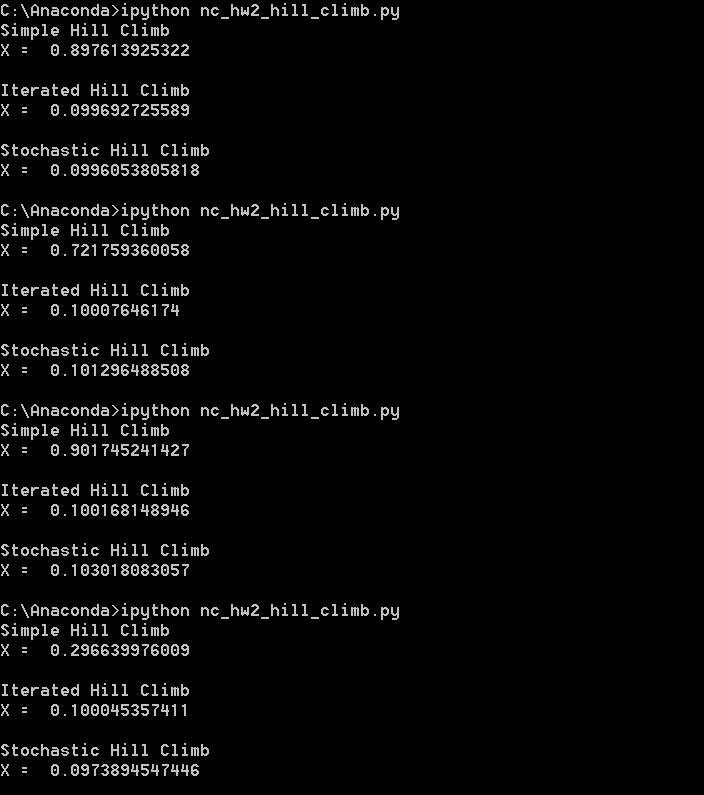
\includegraphics[width=0.75\textwidth]{HillClimb.PNG}
\end{center}
\caption{Sample Hill Climb Algorithms Answers \label{hill_climb} }
\end{figure}


\newpage
\section{Problem 2}
\textbf{Implement and apply the hill-climbing, simulated annealing, and genetic algorithms to maximize function $g(x)$ used in the previous exercise assuming a bitstring representation.} \newline \\
\textbf{Tip: The pertubation to be introduced in the candidate solutions for the hill-climbing and simulated annealing algorithms may be implemented similarly to the point mutation in genetic algorithms. Note that in this case, no concern is required about the domain of x, because the binary representation already accounts for it.} \newline \\
\textbf{Discuss the performance of the algorithms and asses their sensitivity in relation to the input parameters.}

\subsection{Summary}
Expanding on the evaluations in the previous problem we add a simple genetic algorithm to the mix. As mentioned, many of the solutions above can find themselves caught in a local extrema for many optimization problems. The genetic algorithm (granted a large enough initial population) avoids this problem by sampling a larger area of the search space.

\subsection{Implementation}
The code can be found in Listing~\ref{Problem2EA.py}.

\subsubsection{Encoding}
For the gene encoding, we used an unsigned 16 bit integer. This gave us an easy way to store 16 bits. Since we know the domain of the problem is restricted to $[0, 1]$ decoding the genotype into a phenotype was done by dividing the integer value of the bit string by the maximum value of a 16 bit integer (65535). Because the values are stored as integers, we can use numpy's random\_integers function to initialize the population.

\subsubsection{Crossover \& Mutation}
Crossover and mutation were handled by binary operations. Binary masks were stored in lists for each operator and a random index into those lists was generated to pick the mask used.

For mutation the individual was XOR'd with the mask to flip the proper bit. For crossover one parent was AND'd with the chosen mask and the other was AND'd with that masks negation. These values were then OR'd together to make the child individual.

\subsubsection{Selection}
Since our fitness values were simply the y values of the function and maximizing the function was the goal, a simple roulette selection method was chosen.

To avoid having to mess with the list of fitness values, an unused index list is created, and this is what the indexes are chosen from. Iterating through the unused list we add the value at that list to a variable until it is greater than or equal to a random value between 0 and the summation.

Between choosing each index the value at the chosen index is subtracted from the sum to avoid having to sum the unused values again. Unfortunately, since this uses floating point calculations it occasionally didn't reach the sum before the algorithm ran out of indexes. We fixed this problem by defaulting to the last index if the sum hasn't been reached by that point.

\subsection{Analysis}
Through multiple runs with different parameters, it was found that a genetic algorithm could solve this problem consistently with an initial population as low as 10 individuals in 250 iterations. The fastest consistent solution came from runs with around 100 individuals and 100 iterations. If more iterations were run it was able to get more precise, giving an answer of .0999923704891 for a max of .999999956813. Taking into account that the encoding isn't perfect this probably means we have the global max at .1 with a value of 1.


\newpage
\section{Problem 7}
\textbf{Determine, using genetic programming (GP), the computer program (S-expression) that produces exactly the outputs presented in Table 3.3 for each value of x. The following hypotheses are given:}
\begin{itemize}
\item \textbf{Use only functions with two arguments (binary trees).}
\item \textbf{Largest depth allowed for each tree: 4}
\item \textbf{Function set: F = {+, *}}
\item \textbf{Terminal set: T = {0, 1, 2, 3, 4, 5, x}}
\end{itemize}
\centerline{\begin{tabular}{ c c }
\hline
x & Program output \\
\hline
-10 & 153 \\
\hline
-9 & 120 \\
\hline
-8 & 91 \\
\hline
-7 & 66 \\
\hline
-6 & 45 \\
\hline
-5 & 28 \\
\hline
-4 & 15 \\
\hline
-3 & 6 \\
\hline
-2 & 1 \\
\hline
-1 & 0 \\
\hline
0 & 3 \\
\hline
1 & 10 \\
\hline
2 & 21 \\
\hline
3 & 36 \\
\hline
4 & 55 \\
\hline
5 & 78 \\
\hline
6 & 105 \\
\hline
7 & 136 \\
\hline
8 & 171 \\
\hline
9 & 210 \\
\hline
10 & 253 \\
\hline
\end{tabular}}